% Research project report: Bangladesh Food Price Watch (prediction system, stages S22-S33).
% Layout follows the department format (cover, certificate, acknowledgements, abstract, contents, lists of tables and figures, five chapters) and the
% report_sample folder (one main.tex, ref.bib, unilogo.png, figures next to it). Compile with pdfLaTeX + biber (Overleaf default).
% Every number is copied from reports/project/tables/*.csv (file named in the caption) or from reports/project/RESULTS_REGISTER.md; none is computed here.
\documentclass[12pt]{report}

\usepackage[T1]{fontenc}
\usepackage[utf8]{inputenc}
\usepackage{mathptmx}
\usepackage{float}
\usepackage{graphicx}
\graphicspath{{./}{images/}}
\usepackage{amsmath,amssymb,amsfonts}
\usepackage{textcomp}
\usepackage[table]{xcolor}
\usepackage[hidelinks]{hyperref}
\usepackage{url}
\usepackage{ragged2e}
\usepackage{array,multirow}
\usepackage{biblatex}
\ExecuteBibliographyOptions{sorting=none}
\addbibresource{ref.bib}

\usepackage[parfill]{parskip}
\usepackage{geometry}
\usepackage{sectsty}
\chapterfont{\centering}
\geometry{paper=a4paper, top=1in, bottom=1in, left=1.2in, right=0.8in, headheight=0.75cm, footskip=1.5cm, headsep=0.75cm}
\linespread{1.5}
\newcommand{\unexpl}{\emph{not explained by measured cost drivers}}

\begin{document}
\pagenumbering{gobble}
\begin{titlepage}
	\centering
	\begin{figure}[htbp]\centering
\includegraphics[height=4cm,width=4cm]{unilogo.png}\end{figure}
	{\huge\bfseries Comilla University \par}
	\vspace{0.5cm}
	{\scshape\Large\bfseries A RESEARCH PROJECT REPORT \par}
	{\large\textit{on}\par}
	{\scshape\Large\bfseries Bangladesh Food Price Watch: A Price Forecasting and Abnormal-Rise Alert System for Dhaka Retail Food Prices\par}
	\vspace{0.45cm}
	{\scshape\Large\bfseries \textit{Submitted By}\par}
	{\Large\textbf{ROMJAN CHOWDHURY}}\par
	{\Large{Roll No.: 22408024}}\par
	{\Large{Session: 2023--24}}\par
	\vspace{0.35cm}
	{\large\textbf{\textit{In Partial Fulfillment for the Award of}}}\par
	{\Large\textbf{MASTER OF SCIENCE\\}}
	\vspace{0.1cm}
	{\large\textbf{IN }}
	{\large\textbf{COMPUTER SCIENCE AND ENGINEERING}\par}
	\vspace{0.45cm}
	{\Large\textbf{COMILLA UNIVERSITY :: COMILLA-3506}}\par
	\vspace{0.35cm}
	{\Large\bfseries November 2026}\par
\end{titlepage}

\newpage
\begin{center}
    \large\textbf{BONAFIDE CERTIFICATE}\\
\end{center}
\section*{}
Certified that this research project, \textbf{``Bangladesh Food Price Watch: A Price Forecasting and Abnormal-Rise Alert System for Dhaka Retail Food Prices''}, is the bonafide work of \textbf{``Romjan Chowdhury''}, submitted in fulfillment of the requirements of CSE-52, who carried out the project work under my supervision.
\\
\\
\begin{table}[h]
\begin{tabular}{l@{\hspace{3cm}}l}
{Signature} & {Signature} \\
\\
\ldots\ldots\ldots\ldots\ldots\ldots\ldots\ldots\ldots & \ldots\ldots\ldots\ldots\ldots\ldots\ldots\ldots\ldots \\
{Dr. Mahmudul Hasan} & {Dr. Mahmudul Hasan} \\
\textbf{CHAIRMAN OF EXAM COMMITTEE} & \textbf{SUPERVISOR} \\
{Associate Professor} & {Associate Professor} \\
{Department of Computer Science} & {Department of Computer Science} \\
{and Engineering} & {and Engineering} \\
{Comilla University, Cumilla} & {Comilla University, Cumilla} \\
\end{tabular}
\end{table}

\pagenumbering{roman}

\chapter*{ACKNOWLEDGEMENTS}
\addcontentsline{toc}{chapter}{\numberline{}ACKNOWLEDGEMENTS}
First of all, I thank Almighty Allah for the health and patience that let me finish this project.

\noindent I am grateful to my supervisor, \textbf{Dr. Mahmudul Hasan}, Associate Professor, Department of Computer Science and Engineering, Comilla University, for his guidance and for the time he gave to this work, ``Bangladesh Food Price Watch''. His questions about what the results did and did not show shaped how the report is written.

\noindent I also thank the Trading Corporation of Bangladesh, whose published daily price reports are the source of the price data, and the providers of the open driver data: Open-Meteo, the Federal Reserve Bank of St.\ Louis and the market data services behind the exchange-rate series.

\noindent Finally, I thank my family and friends for their support during this work.

\chapter*{ABSTRACT}
\addcontentsline{toc}{chapter}{\numberline{}ABSTRACT}
This project builds a working price watch for the daily retail prices that the Trading Corporation of Bangladesh (TCB) publishes for Dhaka. From 63 items observed over 1,412 report days (May 2021 to October 2026), one LightGBM model forecasts 54 long-history items 1, 7, 14 and 30 report days ahead, gives each forecast an expected range built from the item's own recent errors, flags a price that stays above that range on 3 of the last 5 report days, and splits each alert into the parts attributed to price history, calendar, weather, the Indian onion export measures and the exchange rate. Every setting was fixed on calendar 2024 and written down before the test period (January 2025 to October 2026) was scored once. The forecasts did not beat ``tomorrow equals today'': relative error was 1.010, 1.001, 1.001 and 1.001 at the four horizons, and the model was statistically worse at 1 and 7 report days (Diebold--Mariano $p=0.0001$ and $0.011$). The alert rule, set at the 0.95 level from 2024 false alarms, detected 7 of 12 documented price episodes (11 of 16 product rows), but random dates reached a recall of 0.59 (placebo $p=0.26$), and only 6\% of alert runs started inside an event window. Driver shares changed a lot between refits, so the breakdown is only a rough guide. The pipeline, exports and a dashboard are working, but with these data the forecasts add little to persistence and the alerts are not yet reliable enough to act on.

\newpage
\renewcommand*\contentsname{TABLE OF CONTENTS}
\tableofcontents

\clearpage
\phantomsection
\addcontentsline{toc}{chapter}{\numberline{}LIST OF TABLES}
\listoftables

\clearpage
\phantomsection
\addcontentsline{toc}{chapter}{\numberline{}LIST OF FIGURES}
\listoffigures
\pagenumbering{arabic}

%==================================================================================
\chapter{Introduction}
\justifying

\section{Introduction}
Rice, edible oil, sugar, onion, eggs and lentils take a large share of what a Bangladeshi household spends on food, so a sudden rise in any of them is noticed quickly and often becomes a policy question. The Trading Corporation of Bangladesh (TCB) publishes a retail price report for Dhaka on most working days. The reports are Excel sheets with a minimum and maximum price per item, and they are not available as one clean, machine-readable series.

The TCB prices have a shape that makes forecasting harder than it first looks. A price stays exactly the same on most days and then moves in a step. For administered items such as sugar and edible oil the step follows an announcement. For perishables such as onion and eggs the steps are smaller and more frequent. The median item had an unchanged price on 85 to 93 percent of report days, depending on its group (Table~\ref{tab:strata}). A forecast of ``no change'' is therefore right most of the time, and any model has to beat that to be worth running.

\section{Motivation}
Two kinds of users could use a daily price watch. A person who follows prices wants to know what a staple is likely to cost in a week or a month and how far from that figure a price could reasonably land. A person who follows market behaviour wants to know when a price has risen further than its own recent history makes likely, and whether the cost drivers that can be measured account for that rise. Published forecasting work on Bangladeshi retail prices is thin and mostly uses price history alone \cite{agripricebd}, and I did not find a system that returns the forecast, the range, the alert and the breakdown together for the TCB daily reports.

\section{Problem Statement}
Given the TCB daily retail prices of an item up to a report day, the problem is to forecast its price 1, 7, 14 and 30 report days ahead, to state an expected range around the forecast, to decide whether a price that has risen is outside that range in a way that persists, and to say how much of the model's forecast comes from each measurable driver. The difficulty is that most prices do not move on most days, so a model has to beat the forecast ``tomorrow equals today'' and a good-looking error number alone proves little.

\section{Objectives of the Study}
The objectives are:
\begin{itemize}
    \item to build a clean, audited daily price panel from the TCB reports and join to it the drivers that could be measured, each dated by the day it became known;
    \item to forecast every long-history item at four horizons with one model and to compare that model with five alternatives on a validation year;
    \item to give each forecast an expected range and to raise an alert when the price stays above it, with the alert level fixed from false alarms on non-event days;
    \item to attach a breakdown by driver group to each alert, and to word any residual rise as \unexpl;
    \item to test the settings once on a period that was not used for any choice, and to report the result whether or not it is favourable.
\end{itemize}

\section{Scope of the Study}
The study covers the TCB Dhaka retail reports from 17 May 2021 to 24 October 2026. Of the 63 items, 54 have enough history to forecast; the other nine started in May 2024. Time is counted in report days, because TCB does not publish every day. The 2022 reports are too sparse and are never filled or scored. Forecasting is for the Dhaka retail price only. The study does not claim to find the cause of any price rise, it does not use market-level prices from other sources, and it does not test pretrained forecasting models. The alerts detect an abnormal rise after it has started; they are not an early warning.

\section{Functionality of the Proposed System}
The system takes the price file and produces, for each of the 54 items: a forecast at 1, 7, 14 and 30 report days with a lower and an upper bound; a list of alerts, where an alert starts when the price is above the upper bound on at least 3 of the last 5 report days; and, for each alert day, the contribution of each driver group to the model's forecast and the part of the rise above the range, labelled \unexpl. The results are written to three files (forecasts, alerts and alert drivers) that a Gradio app in a Colab notebook and a local Streamlit dashboard read. A longer price file can be added later and the same steps run again.

\section{Organization of the Report}
This report consists of five chapters.

\textbf{Chapter 1: Introduction} describes the background, problem, objectives, scope and the functions of the system.

\textbf{Chapter 2: Literature Review} reviews related work, states the research gap and lists the contributions.

\textbf{Chapter 3: Methodology} describes the data, the model, its training and the evaluation design.

\textbf{Chapter 4: Experiments and Results} gives the setup and the results for selection, tuning, the sealed test, ranges, alerts and drivers.

\textbf{Chapter 5: Conclusion and Future Work} gives the conclusion, the limitations and the future work.

%==================================================================================
\chapter{Literature Review}

\section{Related Works}
The closest study to this one is a 2026 benchmark on the AgriPriceBD dataset of Bangladeshi market prices. It covers five commodities from July 2020 to June 2025 and compares naive persistence, SARIMA, Prophet, a BiLSTM, Transformer variants and Informer, all using price history only \cite{agripricebd}. No single model was best everywhere. Naive persistence was best for four of the five commodities, and Prophet did badly on step-like prices. That is the same pattern I meet in the TCB data, where the prices stay still for long stretches. Other studies report gains from tree ensembles over a random walk for food price indices in other countries, but I did not read them closely enough to cite them, and they use index or monthly data rather than daily retail prices.

Work on onion markets in Bangladesh shows that imported onion prices strongly influence local onion prices through a non-linear, asymmetric adjustment \cite{onionnardl}. This is the reason the Indian onion export measures are among the drivers here, and the reason each driver is dated by the day it was known.

On the method side the tools are standard. Automatic exponential smoothing is the ETS candidate. LightGBM is a gradient-boosted tree learner that handles mixed numeric inputs and missing values without much preparation \cite{lightgbm}, and its settings were searched with Optuna \cite{optuna}. Forecast error is reported as a ratio to a naive benchmark and in a scale-free form \cite{hk2006}. Two forecasts are compared with the Diebold--Mariano test \cite{dm1995} and its small-sample correction \cite{hln1997}. Whether the share of prices above an upper bound matches its nominal rate is checked with the proportion-of-failures test of Kupiec \cite{kupiec}. The driver breakdown uses the additive per-feature contributions of a tree model, the quantity that SHAP reports for trees \cite{shap}, summed over groups of features. Pretrained forecasting models that accept covariates, such as Chronos-2 \cite{chronos2}, exist but were not tested. Table~\ref{tab:lit} summarises these works and what each is used for here.

\begin{table}[H]\centering\small
\caption{Summary of the literature used in this report.}\label{tab:lit}
\begin{tabular}{|p{2.6cm}|p{3.6cm}|p{5.2cm}|}
\hline
\textbf{Work} & \textbf{Topic} & \textbf{Relevance to this project} \\
\hline
AgriPriceBD benchmark (2026) \cite{agripricebd} & Classical and deep models on Bangladeshi market prices, price history only & Naive persistence was hard to beat; Prophet failed on step-like prices \\
\hline
Mila et al. (2023) \cite{onionnardl} & Spatial price transmission in onion markets, NARDL & Reason for the onion export driver and for dating drivers by availability \\
\hline
Hyndman and Koehler (2006) \cite{hk2006} & Measures of forecast accuracy & Scale-free error and ratio to a naive forecast \\
\hline
Diebold and Mariano (1995) \cite{dm1995}; Harvey et al. (1997) \cite{hln1997} & Test of equal forecast accuracy and its small-sample correction & Test of the model against ``tomorrow equals today'' \\
\hline
Ke et al. (2017) \cite{lightgbm} & LightGBM & The main model \\
\hline
Akiba et al. (2019) \cite{optuna} & Optuna & Search of the model settings on 2024 \\
\hline
Kupiec (1995) \cite{kupiec} & Proportion-of-failures test & Check of the expected range \\
\hline
Lundberg and Lee (2017) \cite{shap} & SHAP, additive feature contributions & Basis of the driver breakdown \\
\hline
Ansari et al. (2025) \cite{chronos2} & Chronos-2, pretrained forecasting with covariates & Not tested; listed as future work \\
\hline
\end{tabular}
\end{table}

\section{Research Gap}
Published forecasting work on Bangladeshi retail prices compares models on a few commodities using price history, and it stops at the point forecast. Three things were missing in what I could find: a forecast with a stated range for each item of a daily retail price report; an alert rule whose level is fixed from false alarms on ordinary days and then checked against documented price episodes; and a way to say, for each alert, how much of the model's forecast comes from the measurable drivers and how much of the rise they leave unexplained. Evidence that external drivers help item-by-item forecasts of Bangladeshi daily retail prices was also not found.

\section{Research Contributions}
The contributions of this project are as follows.
\begin{itemize}
    \item A cleaned and audited daily panel of 63 TCB items over 1,412 report days, with a machine re-read of a 2\% sample against the original sheets that found no mismatch.
    \item A single-model forecasting pipeline for four horizons, compared with five alternatives on a validation year, with every setting fixed on 2024 and written to a committed file before the 2025--26 test was scored once.
    \item An expected-range and alert rule whose level was fixed from 2024 false alarms outside the event windows, and an honest check of it against 12 documented episodes with a random-date control.
    \item A driver breakdown for each alert, with a stability check across refits.
    \item A result that is negative for point forecasts: the model did not beat ``tomorrow equals today'', and the report states this together with the evidence.
    \item A working set of notebooks, export files and a dashboard that run from the raw price file to the alerts and can take a longer price file later.
\end{itemize}

%==================================================================================
\chapter{Methodology}

\section{Dataset Description}

\subsection{Dataset Sources and Collection}
The prices come from the TCB daily retail price reports for Dhaka, downloaded as Excel sheets and converted to one table. Weather comes from Open-Meteo for 13 locations. The exchange rate is the Bangladeshi taka per US dollar, built from two market series spliced at 2 March 2024. The onion export measure comes from a table of Indian export duties, minimum export prices and bans, whose India onion ban dates were checked against the Indian trade notification and press reports. The 12 price episodes used only to score the alerts come from a list of news-documented shocks collected for the earlier study. No driver value is used before the date it became available: weather is lagged five days, and the exchange rate is the last value on or before the report day.

\subsection{Dataset Description}
The price file holds 76,440 rows: 63 items observed over 1,412 report days from 17 May 2021 to 24 October 2026. Each item has a minimum and a maximum price and a unit. The items fall into six groups used for evaluation, plus nine items with short history (Table~\ref{tab:strata}). Nine items started to be reported only in May 2024 and are not forecast, so the model covers 54 items.

\begin{table}[H]\centering\small
\caption{Items by evaluation group. Source: reports/project/tables/P2\_panel\_summary.csv.}\label{tab:strata}
\begin{tabular}{|l|r|r|r|}
\hline
\textbf{Group} & \textbf{Items} & \textbf{Report days} & \textbf{Median share of days with unchanged price} \\
\hline
Imported staples & 19 & 1,412 & 0.932 \\
\hline
Volatile perishables & 10 & 1,412 & 0.874 \\
\hline
Spices & 8 & 1,412 & 0.892 \\
\hline
Administered & 7 & 1,412 & 0.848 \\
\hline
Domestic staples & 7 & 1,412 & 0.906 \\
\hline
Non-food & 3 & 1,412 & 0.918 \\
\hline
Short history (not forecast) & 9 & 591 & 0.928 \\
\hline
\end{tabular}
\end{table}

\subsection{Unique Contribution of the Dataset}
No open, machine-readable daily record of the TCB reports existed that I could find. The panel built here has one row per item and report day, keeps blank and zero prices as not reported, and keeps the 2022 gap visible instead of filling it. It was audited against the original sheets. Because TCB states no reuse terms, the panel and everything derived from it are kept out of the public code repository.

\subsection{Data Preprocessing}
A price of zero or a blank cell means the item was not reported that day, and such cells are never filled in a forecast target. Reporting was irregular in 2022: only 24 reports exist between 12 March and 31 December 2022. That period is never filled, never used as a target and never scored, and any input window that touches it is dropped from training.

I checked the file against the original Excel sheets with a machine re-read of a random 2\% sample: 1,530 item-day rows on 28 report days and 3,060 price cells. No row or cell differed, which puts the transcription error rate below 0.25\% (Wilson 95\% upper limit, Table~\ref{tab:audit}). The audit only checks copying. It cannot show that TCB itself typed a value correctly.

\begin{table}[H]\centering\small
\caption{Audit of the price file against the original TCB sheets. Source: reports/project/tables/P2\_audit\_summary.csv.}\label{tab:audit}
\begin{tabular}{|l|r|}
\hline
\textbf{Measure} & \textbf{Value} \\
\hline
Rows sampled and checked & 1,530 \\
\hline
Report days in the sample & 28 \\
\hline
Price cells checked (minimum and maximum) & 3,060 \\
\hline
Cells that differ & 0 \\
\hline
Cell error rate, Wilson 95\% upper limit & 0.00125 \\
\hline
Row error rate, Wilson 95\% upper limit & 0.0025 \\
\hline
\end{tabular}
\end{table}

For each item and report day $t$, the target at horizon $h \in \{1,7,14,30\}$ is the change in log price between $t$ and $t+h$ report days, defined only if the price at $t+h$ was actually reported. The input price is the last reported price, carried forward, because an item can be skipped on a report day. A driver that is missing stays missing, with a flag, and is never set to zero. A daily driver older than seven days is dropped rather than carried further. The table of exporter events ends on 27 March 2025, so the onion flag is empty for every report day after that, which covers most of the test period.

\section{Model Architecture}

\subsection{LightGBM}
The main model is a LightGBM gradient-boosted tree regressor \cite{lightgbm}. One model is fitted for all items and all four horizons, using rows of the four horizons stacked together with the horizon as an input. A forecast is the last price times the exponential of the predicted change, so the model works in log changes and its errors do not depend on the price level of the item.

\subsection{Model Inputs}
The model uses 25 inputs in five groups (Table~\ref{tab:features}). The price-history inputs are the log price, log changes over 1, 7, 14 and 30 report days, the deviation of the price from its 30-report mean, the 30-report volatility of one-day changes, and the number of reports since the price last changed, together with item and group codes and the horizon. The calendar inputs are the month, the day of the week, the days to Ramadan and to the two Eids, a Ramadan flag, holidays in the coming week and the days since the previous report. The weather inputs are the 7-day maximum temperature, the 30-day mean temperature and the 7-day rainfall for seven items. The onion export flag covers the two onion items. The exchange rate, as a level and a 30-day change, covers 34 items (imported staples, administered items and spices).

\begin{table}[H]\centering\small
\caption{Model inputs by driver group. Source: reports/project/tables/P3\_driver\_inventory.csv and config/project.yaml.}\label{tab:features}
\begin{tabular}{|p{3cm}|p{7cm}|p{2.5cm}|}
\hline
\textbf{Group} & \textbf{Inputs} & \textbf{Items with a value} \\
\hline
Price history & log price, log changes, deviation from rolling mean, rolling volatility, reports since change, item and group codes, horizon & all 54 \\
\hline
Calendar & month, weekday, days to Ramadan and each Eid, Ramadan flag, holiday in next 7 days, days since previous report & all 54 \\
\hline
Weather & 7-day maximum temperature, 30-day mean temperature, 7-day rainfall & 7 \\
\hline
Onion export measure & 1 while an Indian onion export duty, price floor or ban is in force & 2 \\
\hline
Exchange rate & log taka per dollar, 30-day change & 34 \\
\hline
\end{tabular}
\end{table}

\subsection{Candidate Models}
Six models were compared on the validation year. The naive model forecasts no change and is the yardstick. Automatic ETS is fitted to each item's own log price; for an item with fewer than 30 observations at an origin it falls back to no change. Ridge regression and a random forest use the same inputs as LightGBM. The LSTM reads the last 30 log prices together with calendar and price-history inputs and an item embedding, and it was trained for a small number of epochs on the CPU.

\subsection{Expected Range and Alert Rule}
The expected range at horizon 7 comes from each item's own forecast errors. At a forecast origin, the item's last 120 errors whose target date had already passed are taken, and the 5th and 95th percentiles of those errors give the lower and upper bounds. An alert starts when the price is above the upper bound on at least 3 of the last 5 report days, and a run of consecutive alert days counts as one alert. The percentile used for the upper bound (the alert level) is chosen from 0.90, 0.95, 0.975 and 0.99 as the lowest one that gives at most 2 false alarms per item-year on 2024 days outside the event windows.

\subsection{Driver Breakdown}
The per-feature contributions of the model to a forecast are added up within each driver group (price history, calendar, weather, onion export measure, exchange rate). The same sums are made for all items, for each item group, and for each alert day. As a stability check, three models fitted with data up to different report days (1011, 1211 and 1411) were compared on the same rows. The part of a rise above the upper bound is reported as \unexpl; this describes the model's inputs only and says nothing about who or what caused the rise.

\section{Model Training and Optimization}

\subsection{Training Strategy}
At a forecast origin the model sees only rows whose target date lies on or before the origin, so nothing from the future enters training. The window is expanding. The model is refitted every 8 forecast origins, where origins are 7 report days apart, and it is reused between refits. Rows that touch the 2022 gap are removed from training.

\subsection{Loss Function}
The objective was part of the search: L1 (absolute error), Huber or L2. L1 was chosen, which matches the main metric, the mean absolute error of the log price change.

\subsection{Hyperparameter Search}
Optuna \cite{optuna} with a tree-structured sampler (seed 42) ran 50 trials. Each trial was scored on 31 origins from January to August 2024. The best setting was then compared with the default on 9 origins from October to November 2024 and kept only if it was better there. The 2025--26 test period was not touched in either step.

\subsection{Training Configuration}
Table~\ref{tab:params} lists the chosen setting. The test uses exactly this setting and the 25 inputs above.

\begin{table}[H]\centering\small
\caption{Chosen LightGBM setting. Source: state/tuning\_S26.json and reports/project/tables/P6\_tuning\_trials.csv.}\label{tab:params}
\begin{tabular}{|l|r|}
\hline
\textbf{Parameter} & \textbf{Value} \\
\hline
Objective & L1 \\
\hline
Number of trees & 400 \\
\hline
Learning rate & 0.0196 \\
\hline
Leaves per tree & 6 \\
\hline
Minimum rows per leaf & 76 \\
\hline
Feature fraction & 0.665 \\
\hline
Bagging fraction & 0.846 \\
\hline
L1 penalty & 7.44 \\
\hline
L2 penalty & 1.99 \\
\hline
\end{tabular}
\end{table}

\section{Model Evaluation}

\subsection{Validation and Test Design}
Calendar 2024 is the validation year. Six candidates were compared on 43 forecast origins in 2024, spaced 7 report days apart. The naive forecast is the yardstick and cannot be chosen, and a simpler model is preferred if it is within 1\% of the best. Before the test was scored, the chosen settings, the 25 inputs, the list of metrics and the list of checks were written to a file and committed to the repository (state/prereg\_S27.yaml), and the code refuses to score the test unless that file is committed. The test has 87 forecast origins, again 7 report days apart, from January 2025 to October 2026, with the model refitted every 8 origins. Two further schemes check the main result: walk-forward on 2023 and 2024, and a sliding window of the latest 500 report days. The test was scored once. The 2025--26 period had already been scored by an earlier version of this study, so it is not a first look at that data.

\subsection{Forecast Metrics}
The primary metric is the mean absolute error of the log price change, which is about the percentage error. For each item I divide the model's error by the naive error and summarise the ratio over items with a geometric mean, where 1 means a tie with ``tomorrow equals today'' and values above 1 mean the model is worse. I also report the absolute error in taka, the error on days where the price changed against days where it did not, the direction accuracy on days the price moved, the coefficient of determination on the price changes, and the Diebold--Mariano test of the model against the naive forecast.

\subsection{Range and Alert Evaluation}
For the ranges I report how often the price was below the upper bound and inside the central interval, the average width, and the Kupiec test of the exceedance rate \cite{kupiec}. For the alerts I use the 12 documented episodes. An episode window runs from 14 days before the recorded onset to 30 days after the news peak, and an episode counts as detected if an alert starts inside the window for at least one affected item. I report recall, precision (the share of alert runs that start inside a window), false alarms per item-year in 2024 outside the windows, and a random-date control in which each episode window is moved to a random start in the evaluation period, 300 times. The alert level is fixed and committed (state/prereg\_S28.yaml) before any episode is scored. The model is never trained on events and the level is never tuned on them.

%==================================================================================
\chapter{Experiments and Results}

\section{Introduction}
This chapter reports the experiments in the order the system runs them: the setup, the data actually used, model selection and tuning on 2024, the sealed test, the expected ranges, the alerts, the driver breakdown, an example of the output, and a discussion.

\section{Experimental Setup}

\subsection{Hardware Configuration}
Data preparation, the audit and the dashboard ran on a personal Windows computer. All model fitting ran on Google Colab with a CPU runtime and no accelerator, limited to two threads in the fits (Table~\ref{tab:hardware}).

\begin{table}[H]\centering\small
\caption{Hardware configuration.}\label{tab:hardware}
\begin{tabular}{|l|p{8cm}|}
\hline
\textbf{Component} & \textbf{Details} \\
\hline
Work computer & Windows 10; data conversion, audit, unit tests, local dashboard \\
\hline
Model fitting & Google Colab, CPU runtime, no GPU; two threads used by the fits \\
\hline
Storage & Google Drive folder for data, results and models; GitHub repository for code \\
\hline
\end{tabular}
\end{table}

\subsection{Software Environment}
Table~\ref{tab:software} lists the tools. The Colab notebooks clone the code from GitHub at each start, so the code is not stored on Drive.

\begin{table}[H]\centering\small
\caption{Software environment.}\label{tab:software}
\begin{tabular}{|l|p{8cm}|}
\hline
\textbf{Tool} & \textbf{Use} \\
\hline
Python 3.13 (Colab) & all stages \\
\hline
pandas, pyarrow & price panel and feature tables \\
\hline
LightGBM & main model \\
\hline
Optuna & tuning, 50 trials \\
\hline
statsforecast (AutoETS) & ETS candidate \\
\hline
scikit-learn & ridge and random forest candidates \\
\hline
PyTorch (CPU) & LSTM candidate \\
\hline
Gradio, Streamlit & dashboard in Colab and on the work computer \\
\hline
pytest & unit tests and stage acceptance checks \\
\hline
\end{tabular}
\end{table}

\subsection{Implementation Details}
Six Colab notebooks run the stages in order: data and features; model selection and tuning; the sealed test; alerts and drivers; the production fit and export; and a notebook that shows the exports and downloads them. Each stage writes its results to Google Drive and records a hash of every output, so a stage that has finished is skipped on a rerun, and a dropped runtime resumes from the saved pieces. The test is guarded by a seal record that allows one scoring per committed pre-registration. A rerun after the 2025--26 test had already been scored reused the saved forecasts and the same seal, and reproduced the same numbers.

\section{Dataset Description}

\subsection{Dataset Distribution}
Table~\ref{tab:strata} shows the items by group. The model uses 54 items. For the validation year there were 43 origins from 2024-01-01 to 2024-11-24, and for the test 87 origins from January 2025 to October 2026.

\subsection{Price Change Frequency}
The share of forecasts where the price actually changed rises with the horizon (Table~\ref{tab:test}). At 1 report day ahead the price changed in 6.9\% of the cases, at 7 in 25.6\%, at 14 in 37.7\% and at 30 in 52.4\%. This is the main property of the data: at the short horizons almost every correct forecast is ``no change''.

\section{Training and Tuning Results}

\subsection{Model Selection on 2024}
No candidate beat the naive forecast on the 2024 validation origins (Table~\ref{tab:select}). ETS came closest, at 5\% worse than naive overall, LightGBM was 17\% worse, and ridge regression was worst. Because the naive forecast cannot be chosen, ETS was the nominal winner. The explanation step needs a tree model, so I kept LightGBM as the main model and logged that decision, with this table, before tuning. The model was therefore not chosen because it won the comparison, and the results below should be read with that in mind.

\begin{table}[H]\centering\small
\caption{Validation on 2024, 43 origins, all four horizons. Lower is better; relative error 1.000 is a tie with ``tomorrow equals today''. Source: reports/project/tables/P5\_model\_selection\_overall.csv.}\label{tab:select}
\begin{tabular}{|l|r|r|}
\hline
\textbf{Model} & \textbf{Error of log change} & \textbf{Relative to naive} \\
\hline
Naive (tomorrow = today) & 0.0231 & 1.000 \\
\hline
ETS & 0.0235 & 1.053 \\
\hline
LightGBM & 0.0241 & 1.173 \\
\hline
LSTM & 0.0245 & 1.378 \\
\hline
Random forest & 0.0272 & 1.698 \\
\hline
Ridge regression & 0.0292 & 2.316 \\
\hline
\end{tabular}
\end{table}

\subsection{Tuning}
Across the 50 trials the best score on the tuning origins was 0.02478 and the median trial was 0.02486, so most settings that were not clearly bad ended up almost the same. The default setting scored 0.02592 on the tuning origins and 0.02050 on the confirmation origins; the best trial scored 0.02478 and 0.01969. The tuned model is small (Table~\ref{tab:params}). The tuning found a better setting, and it also found one that moves the forecast very little from zero.

\subsection{Learning Curve}
Over 400 trees the training error went from 0.0305 to 0.0302, and the error on a holdout of the latest 15\% of report days did not improve (0.0171 to 0.0172, Figure~\ref{fig:lc}). Adding trees gave the model nothing more to learn from these inputs.

\begin{figure}[H]\centering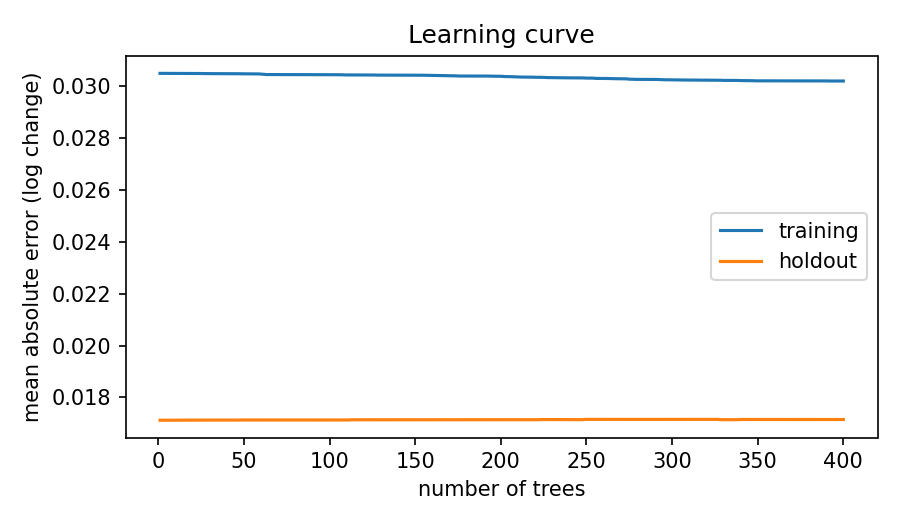
\includegraphics[width=0.7\textwidth]{F13_learning_curve.png}\caption{Training and holdout error by number of trees. Source: reports/project/figures/F13.}\label{fig:lc}\end{figure}

\section{Evaluation Results}

\subsection{Test Accuracy}
On the sealed test the model matches the naive forecast closely and does not beat it at any horizon (Table~\ref{tab:test}, Figure~\ref{fig:rel}). The geometric-mean relative error is 1.0096, 1.0013, 1.0009 and 1.0007 at horizons 1, 7, 14 and 30. At horizons 1 and 7 the model is worse by a margin that is small in size but clear in the Diebold--Mariano test ($p=0.0001$ and $0.011$); at horizons 14 and 30 there is no detectable difference ($p=0.92$ and $0.50$).

The reason is visible in the error split. Most of the error comes from days when the price moved: at horizon 7 the error is 0.0467 on days the price changed and 0.0001 on days it did not, and the price changed on 26\% of those forecasts. The model predicts almost no change, so it is nearly perfect on unchanged days and about as wrong as the naive forecast on changed ones. The coefficient of determination on the price changes is between $-0.002$ and $0.012$. Direction is right on only 15\% to 38\% of the days where the price moved, which is what a forecast of no change would give.

\begin{table}[H]\centering\small
\caption{Sealed test, January 2025 to October 2026, 87 origins. Relative error is the geometric mean over 54 items of model error divided by naive error. Sources: reports/project/tables/P7\_accuracy\_by\_horizon.csv and P7\_dm\_vs\_naive.csv.}\label{tab:test}
\begin{tabular}{|r|r|r|r|r|r|r|}
\hline
\textbf{Horizon} & \textbf{Model error} & \textbf{Naive error} & \textbf{Relative error} & \textbf{Error (Tk)} & \textbf{Price changed} & \textbf{DM $p$} \\
\hline
1 & 0.0028 & 0.0027 & 1.0096 & 3.1 & 0.069 & 0.0001 \\
\hline
7 & 0.0120 & 0.0120 & 1.0013 & 23.8 & 0.256 & 0.011 \\
\hline
14 & 0.0199 & 0.0199 & 1.0009 & 43.2 & 0.377 & 0.92 \\
\hline
30 & 0.0323 & 0.0324 & 1.0007 & 79.2 & 0.524 & 0.50 \\
\hline
\end{tabular}
\end{table}

\begin{figure}[H]\centering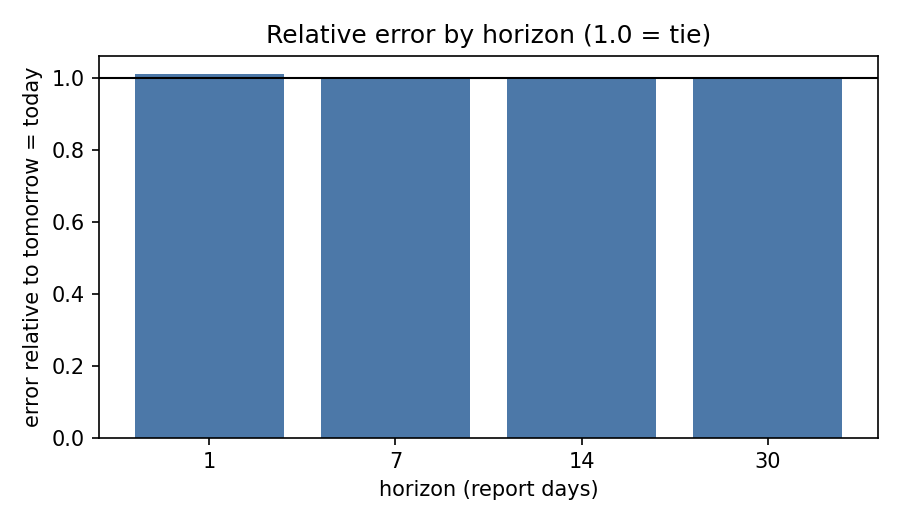
\includegraphics[width=0.7\textwidth]{F10_relative_error_by_horizon.png}\caption{Relative error by horizon on the test (1.0 is a tie with ``tomorrow equals today''). Source: reports/project/figures/F10.}\label{fig:rel}\end{figure}

\subsection{Results by Item Group and Item}
Item by item the picture is the same. Out of 54 items, the model had a lower error than the naive forecast for 13 items at horizon 7, 13 at horizon 14 and 16 at horizon 30, and the ratio ranged from 0.96 to 1.03 (P7\_accuracy\_by\_item.csv). By group, the ratio was between 0.998 and 1.017 everywhere (Table~\ref{tab:group}). The only group-and-horizon cells below 1 are administered items at 30 days (0.999) and volatile perishables at 14 and 30 days (0.999 and 0.998), and these differences are far too small to count as evidence.

\begin{table}[H]\centering\small
\caption{Relative error to the naive forecast by item group and horizon on the test (geometric mean over items). Source: reports/project/tables/P7\_accuracy\_by\_group.csv.}\label{tab:group}
\begin{tabular}{|l|r|r|r|r|}
\hline
\textbf{Group} & \textbf{h = 1} & \textbf{h = 7} & \textbf{h = 14} & \textbf{h = 30} \\
\hline
Administered & 1.008 & 1.001 & 1.001 & 0.999 \\
\hline
Domestic staples & 1.017 & 1.004 & 1.002 & 1.002 \\
\hline
Imported staples & 1.003 & 1.001 & 1.001 & 1.002 \\
\hline
Non-food & 1.001 & 1.000 & 1.001 & 1.002 \\
\hline
Spices & 1.014 & 1.001 & 1.000 & 1.001 \\
\hline
Volatile perishables & 1.017 & 1.003 & 0.999 & 0.998 \\
\hline
\end{tabular}
\end{table}

\subsection{Robustness Checks}
The two further schemes give the same answer, and the older walk-forward years are worse for the model (Table~\ref{tab:wf}). In 2023 the model was 11\% worse than naive at horizon 1 and 3\% worse at the other horizons. The sliding-window version was a little worse than the expanding window on the test.

\begin{table}[H]\centering\small
\caption{Relative error to the naive forecast under the other evaluation schemes. Source: reports/project/tables/P7\_walk\_forward.csv.}\label{tab:wf}
\begin{tabular}{|l|r|r|r|r|}
\hline
\textbf{Scheme} & \textbf{h = 1} & \textbf{h = 7} & \textbf{h = 14} & \textbf{h = 30} \\
\hline
Rolling origin 2025--26 (main) & 1.0096 & 1.0013 & 1.0009 & 1.0007 \\
\hline
Walk-forward 2023 & 1.1143 & 1.0294 & 1.0272 & 1.0253 \\
\hline
Walk-forward 2024 (tuning year) & 1.0343 & 1.0047 & 1.0027 & 1.0027 \\
\hline
Sliding window of 500 reports & 1.0270 & 1.0078 & 1.0077 & 1.0047 \\
\hline
\end{tabular}
\end{table}

\subsection{Error Analysis}
The error analysis (P7\_error\_analysis.csv) shows no difference between normal periods and the weeks around Ramadan and the Eids beyond a slightly larger error in the latter for both the model and the naive forecast (0.0126 against 0.0119 at horizon 7). The bias, meaning the mean of forecast minus actual in log terms, is close to zero (mean $-0.00008$ across origins at horizon 7, Figure~\ref{fig:bias}). The largest forecast errors are mostly for ginger in January 2025 at the 30-day horizon, with a log error of up to 1.4, and for potato and local onion at 30 days. Figure~\ref{fig:dist} shows the error distribution at horizon 7, and Figure~\ref{fig:avf} shows actual and forecast prices for five items; the two lines are close because the forecast is almost always the last price.

\begin{figure}[H]\centering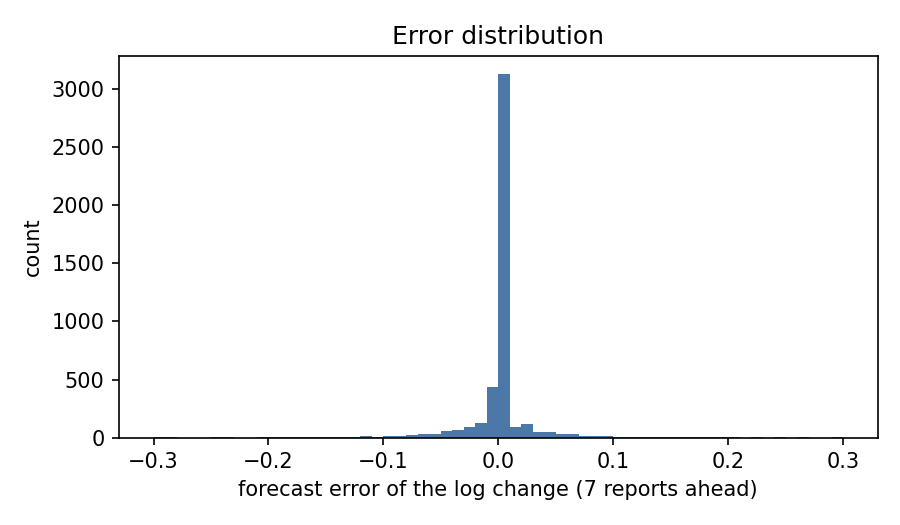
\includegraphics[width=0.7\textwidth]{F11_error_distribution.png}\caption{Distribution of the forecast error of the log change, 7 report days ahead (errors clipped at $\pm0.3$). Source: reports/project/figures/F11.}\label{fig:dist}\end{figure}

\begin{figure}[H]\centering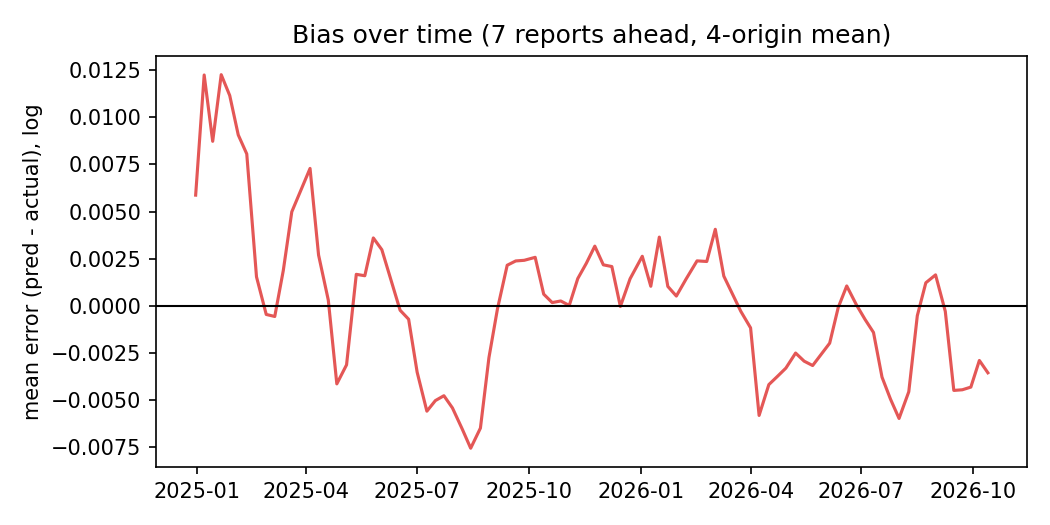
\includegraphics[width=0.75\textwidth]{F12_bias_over_time.png}\caption{Bias over time at horizon 7 (four-origin mean). Source: reports/project/figures/F12.}\label{fig:bias}\end{figure}

\begin{figure}[H]\centering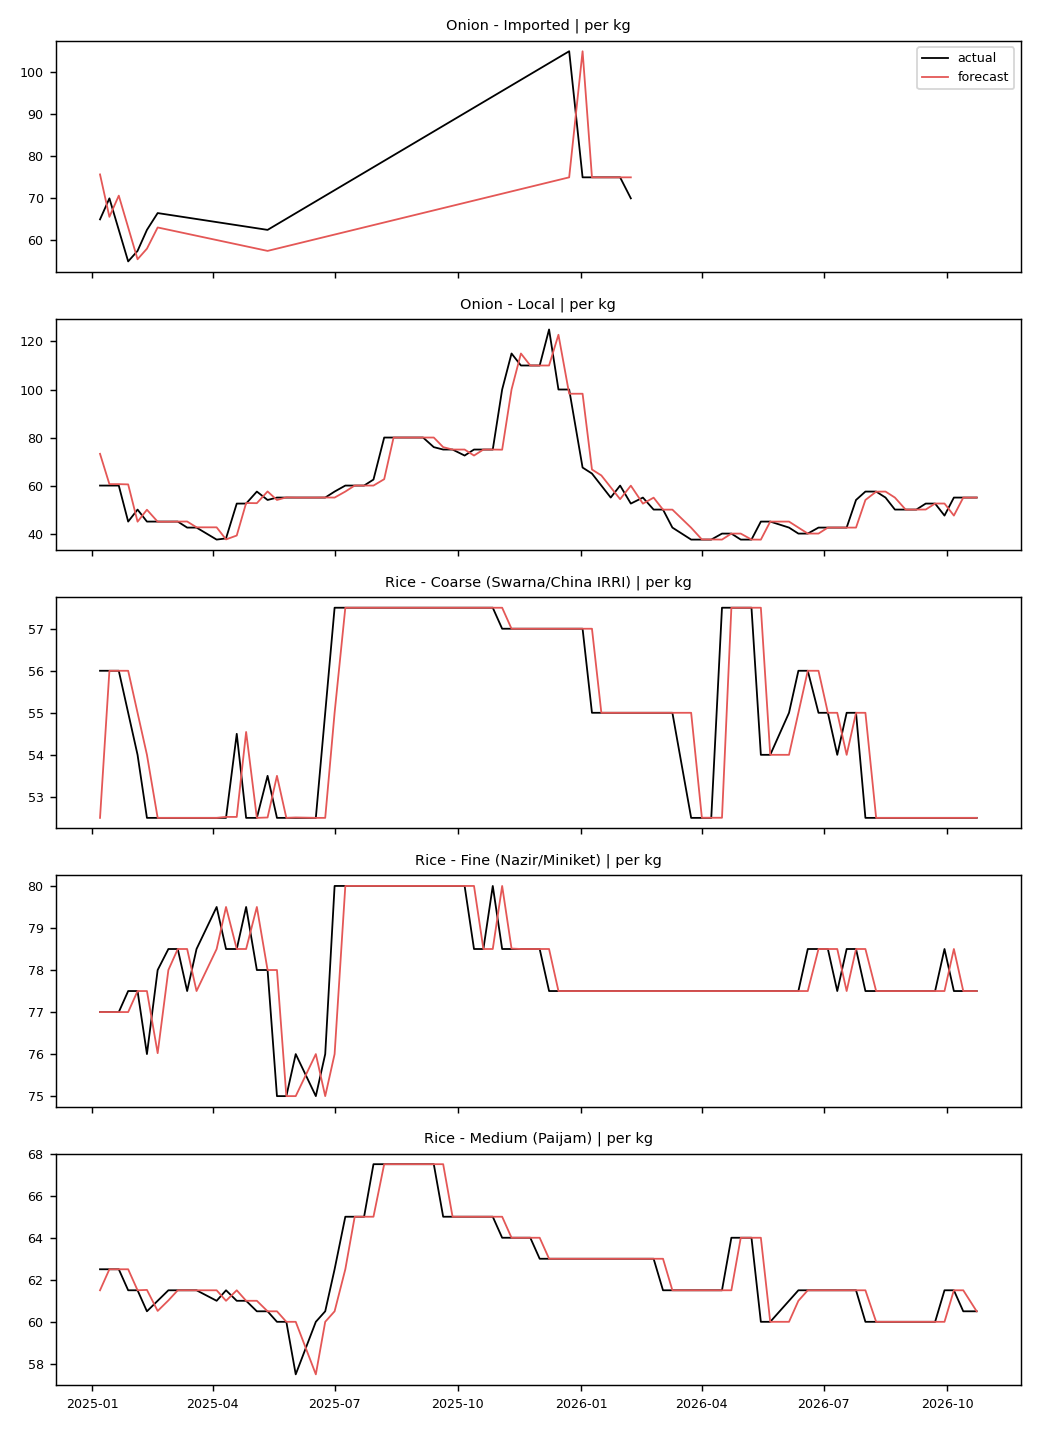
\includegraphics[width=0.85\textwidth]{F14_actual_vs_forecast.png}\caption{Actual and forecast prices at horizon 7 for five items on the test. Source: reports/project/figures/F14.}\label{fig:avf}\end{figure}

\subsection{Expected Ranges}
At horizon 7, over 55,337 daily forecasts from June 2023 to October 2026, the upper bound at the 0.95 level was exceeded on 5.9\% of days, against 5\% expected, so the upper bound covered 0.941 of the outcomes. The central interval between the 5th and 95th percentiles covered 0.883 against 0.90 expected. The Kupiec test rejects the nominal rate ($p<0.001$), but with this many dependent observations the test is strict, and the practical gap is under one percentage point on the upper side. The result was similar in the two periods (upper coverage 0.939 in 2023--24 and 0.943 in 2025--26), and the bound was narrower in the second period (mean width 0.088 against 0.121 in log terms). The ranges are slightly too tight, not badly so.

\subsection{Alerts}
Table~\ref{tab:level} shows how the alert level was chosen. At the 0.90 level there were 3.07 false alarms per item-year in 2024 outside the event windows, which is over the target of 2, and 0.95 was the lowest level under it (1.92). Level 0.95 was therefore fixed, and the scoring of the episodes came after that.

\begin{table}[H]\centering\small
\caption{Alert levels. False alarms are alert runs per item-year in 2024 outside event windows; recall and precision are over the whole period, counted by product row. Source: reports/project/tables/P8\_level\_curve.csv.}\label{tab:level}
\begin{tabular}{|r|r|r|r|r|}
\hline
\textbf{Level} & \textbf{False alarms, 2024} & \textbf{Event recall} & \textbf{Precision} & \textbf{Alert runs} \\
\hline
0.90 & 3.07 & 0.688 & 0.061 & 635 \\
\hline
0.95 (chosen) & 1.92 & 0.688 & 0.061 & 429 \\
\hline
0.975 & 1.63 & 0.625 & 0.054 & 368 \\
\hline
0.99 & 1.44 & 0.500 & 0.052 & 327 \\
\hline
\end{tabular}
\end{table}

At the chosen level, alerts started inside the window of 7 of the 12 episodes (11 of 16 product rows; Table~\ref{tab:events}). The misses are the sugar episode of June 2023, two potato episodes in 2024, the egg episode of October 2024 and the green chilli episode of July 2026. The negative lead times in the table should not be read as early warning. The windows open 14 days before the recorded onset and can run for months after the news peak (the rice episode runs to June 2025), so an alert that starts anywhere inside counts as a detection. The long windows also help the detection rate, since a single alert run anywhere inside a 600-day window is enough.

The random-date control puts the detection rate in perspective. When each episode's window was moved to a random start inside the evaluation period, the mean recall was 0.59, against 0.69 observed, and 26\% of the random draws did as well or better ($p=0.26$ over 300 draws). So the alerts are not distinguishable from chance on these 12 episodes. Of 429 alert runs, only 6\% (26 runs) began inside an event window; the others were not matched to any of the documented episodes. Some of these may be real rises that were not in the news-based list, but the list is the only reference I have, and the system cannot tell the two cases apart.

\begin{table}[H]\centering\small
\caption{The 12 documented episodes and whether an alert started inside the window (level 0.95). Lead is the number of days between the first alert and the news peak, negative if before. Source: reports/project/tables/P8\_event\_scores.csv.}\label{tab:events}
\begin{tabular}{|l|l|l|l|r|r|}
\hline
\textbf{Episode} & \textbf{Product} & \textbf{Onset} & \textbf{News peak} & \textbf{Detected} & \textbf{Lead (days)} \\
\hline
BD-S09 & Sugar & 2023-06-01 & 2023-06-25 & no & -- \\
\hline
BD-S11 & Eggs (farm) & 2023-08-01 & 2023-08-13 & yes & 0 \\
\hline
BD-S12 & Onion (imported, local) & 2023-08-01 & 2023-08-21 & yes & $-4$ \\
\hline
BD-S13 & Onion (imported, local) & 2023-10-01 & 2023-12-09 & yes & $-38$ \\
\hline
BD-S14 & Potato & 2023-10-01 & 2023-11-13 & yes & $-12$ \\
\hline
BD-S15 & Rice (coarse, medium) & 2023-10-01 & 2025-06-10 & yes & $-558$ \\
\hline
BD-S16 & Eggs (farm) & 2024-05-01 & 2024-05-19 & yes & $-11$ \\
\hline
BD-S17 & Potato & 2024-07-01 & 2024-08-18 & no & -- \\
\hline
BD-S19 & Potato & 2024-09-01 & 2024-09-05 & no & -- \\
\hline
BD-S20 & Eggs (farm) & 2024-10-01 & 2024-10-18 & no & -- \\
\hline
BD-S21 & Soybean oil (bottled, loose) & 2024-10-01 & 2025-02-09 & yes & $-125$ \\
\hline
BD-S22 & Green chilli & 2026-07-01 & 2026-07-31 & no & -- \\
\hline
\end{tabular}
\end{table}

\subsection{Driver Breakdown}
On the last 120 report days, price history accounts for 56\% of the average size of the model's contributions, the exchange rate for 17\%, the calendar for 14\%, the onion export measure for 10\% and weather for 4\% (Table~\ref{tab:drivers}). Because the model forecasts nearly zero change, these are shares of small numbers. They describe what the model leans on, not how much a driver moved a price. The shares look similar across item groups, with price history at 46\% to 68\% in every group, and the exchange rate larger for non-food items and spices (about 24\% and 22\%).

\begin{table}[H]\centering\small
\caption{Share of the average absolute contribution by driver group, last 120 report days. Source: reports/project/tables/P9\_driver\_overall.csv and P9\_driver\_stability.csv.}\label{tab:drivers}
\begin{tabular}{|l|r|r|r|r|}
\hline
\textbf{Group} & \textbf{Final model} & \textbf{Fitted to day 1211} & \textbf{Fitted to day 1011} & \textbf{Spread} \\
\hline
Price history & 0.556 & 0.359 & 0.241 & 0.315 \\
\hline
Exchange rate & 0.170 & 0.017 & 0.102 & 0.153 \\
\hline
Calendar & 0.138 & 0.009 & 0.122 & 0.130 \\
\hline
Onion export measure & 0.096 & 0.008 & 0.067 & 0.088 \\
\hline
Weather & 0.040 & 0.607 & 0.468 & 0.567 \\
\hline
\end{tabular}
\end{table}

The breakdown is not stable. The model fitted to data up to report day 1211 gave weather 61\% and price history 36\%, and the model fitted to day 1011 gave weather 47\%. The final model gives weather 4\%. A tool that moves this much between refits cannot be used to say what drives a price, and I describe the drivers as helpful for specific items, not proven. Two sign checks were planned. The price-above-recent-mean input has the expected sign (correlation $-0.18$ with its contribution, meaning a price high against its recent mean pulls the forecast down). The exchange-rate check returned no value and I did not find out why in the time available. At horizons 1 and 7 the shares are identical to many decimals, which fits a model whose trees never split between those two horizons, in line with the finding that it forecasts almost no change.

\section{Sample Input and Output}

\subsection{Input}
The input is the price file up to the last report day, 24 October 2026, and the driver files. For a given item the model uses the last reported price, its recent changes and volatility, the calendar position and, where the item has them, weather and the exchange rate.

\subsection{Forecast and Range}
For broiler chicken the last reported price was 185 Tk. The 1-report-day forecast was 185 Tk with a range from 179.4 to 190.4 Tk. For small cardamom, last price 5,100 Tk, the 1-report-day forecast was 5,100 Tk with a range from 5,099.3 to 5,135.9 Tk. For the loose atta price of 50 Tk the range at horizon 1 collapses to a single value, 50 Tk. These are rows of the production export, which holds 216 forecasts (54 items at four horizons).

\subsection{Alert and Driver Breakdown}
For each alert day the export file lists the contribution of each driver group, the expected change, and the part of the rise above the upper bound with the note that it is \unexpl. There are 429 alert runs and 3,081 alert days in the export. The note describes the model's inputs only; it does not say that anyone caused a rise.

\subsection{Dashboard}
A local Streamlit dashboard and a Gradio app in Colab read the three export files. They show the forecast and range for a chosen item, the recent alerts, and the driver chart for an alert day. Both state on the first screen that the alerts are not an early warning and that the model did not beat ``tomorrow equals today'' on the test.

\section{Discussion}
The main result is that the forecasts add nothing to persistence on these data. The prices change on few days, the model's best move is to predict no change, and the inputs I could measure did not predict the days when a price does change. The ETS and LightGBM results on 2024 and the walk-forward checks point the same way, and the learning curve shows the model has little to learn from its inputs. This agrees with the AgriPriceBD benchmark, where naive persistence was best for four of five commodities \cite{agripricebd}, so it is not a flaw of one model.

The ranges are usable as an expected band, since the upper bound is exceeded close to the nominal rate, but they are narrow because the model forecasts little movement. The alerts are weaker than the ranges suggest. The detection rate of 7 of 12 episodes is no better than random dates, only 6\% of alert runs lie inside a documented episode, and the long episode windows make detection easy. The system can flag unusual rises for a person to look at; it cannot yet say which flagged rises matter. The driver breakdown is the least reliable part, because its shares change a great deal when the model is refitted.

What can be relied on is the process: the settings were fixed before the test, the test was scored once, a rerun reproduced the same numbers, and every number in this report is listed in a results register with its file and command.

%==================================================================================
\chapter{Conclusion and Future Work}

\section{Conclusion}
This project delivered a price watch for TCB Dhaka retail prices that runs from the raw price file to forecasts, expected ranges, alerts and a driver breakdown, and the evidence says it is not yet useful for forecasting: on the 2025--26 test one LightGBM model was no better than ``tomorrow equals today'' at 1, 7, 14 or 30 report days, and slightly worse at the shortest two, because most TCB prices do not change on most days and the inputs I could measure did not predict the days when they do. The ranges came close to their nominal coverage and the alert rule, fixed on 2024 data, flagged 7 of 12 documented price episodes, but random dates did almost as well and about 94\% of alert runs were not tied to any documented episode, so the alerts should be read as a way to review unusual rises and not as a warning. The driver shares changed too much between refits to support claims about causes, and the fair summary is that the measured drivers were not shown to explain these prices.

\section{Limitations}
This research has several limitations that should be acknowledged:
\begin{itemize}
    \item \textbf{Forecast value}: on these data the forecasts add nothing over persistence at any horizon, so the value of the system rests on its ranges, alerts and bookkeeping, and the alerts are weak.
    \item \textbf{Model choice}: LightGBM was kept for the driver breakdown although it did not win the 2024 comparison, so a different choice might have done somewhat better, although the ETS result suggests not by much.
    \item \textbf{Test period}: the 2025--26 period was not a first look, because an earlier version of this study had scored it. The settings were fixed before this run, but that earlier exposure cannot be undone.
    \item \textbf{Number of episodes}: twelve episodes is a small number, and five of them fall in 2024, the year used to set the level (the level was set from non-event days only, so the episodes did not influence it). A recall of 7 of 12 has a wide uncertainty band and the random-date comparison has little power. The episode windows are long, which flatters detection, and the list may be missing real rises that would turn some of the 94\% of unmatched alert runs into correct ones.
    \item \textbf{Data gaps}: the 2022 reports are too sparse and are not used. The table of Indian onion export measures ends in March 2025, so the onion input is empty after that date. Weather and exchange-rate files end a few days before the end of the price file, which will matter when new reports are added.
    \item \textbf{Audit}: the audit covers copying only, and it was run on the extended price file whereas the model uses the file to 24 October 2026.
    \item \textbf{Data terms}: TCB does not state terms for reusing its reports, so the price data and everything derived from it are kept out of the public repository, and the Gradio link of the dashboard is public while it runs.
    \item \textbf{Driver breakdown}: it has no independent check beyond two sign tests, one of which returned no value, and its shares change a great deal between refits.
\end{itemize}

\section{Future Work}
Several directions follow from this work:
\begin{itemize}
    \item \textbf{Change versus no change}: model separately whether a price will change and by how much, which the step-like prices suggest.
    \item \textbf{Episodes}: build a larger and independently checked list of price episodes, with shorter windows, so that alert detection can be tested with more power.
    \item \textbf{Onion export table}: extend the table of Indian export measures beyond March 2025.
    \item \textbf{Market-level prices}: use WFP market prices to test whether a rise is national, regional or local.
    \item \textbf{Pretrained models}: test a pretrained forecasting model that accepts covariates, such as Chronos-2 \cite{chronos2}, under a new pre-registration.
    \item \textbf{Stable explanations}: use a method that keeps driver shares steady across refits before using them to describe a rise.
\end{itemize}

\begingroup
\let\clearpage\relax
\renewcommand{\bibname}{REFERENCES}
\addcontentsline{toc}{chapter}{\numberline{}REFERENCES}
\printbibliography
\endgroup

\end{document}
